% Generated from work/deck/chart-data-en.mjs; numeric data preserved.
% Input in a column; rocpr is intended for full frame width.
\begingroup
\definecolor{blueplot}{HTML}{4E79A7}
\definecolor{redplot}{HTML}{D95F59}
\definecolor{inkplot}{HTML}{111111}
\definecolor{lightplot}{HTML}{8FB8DA}
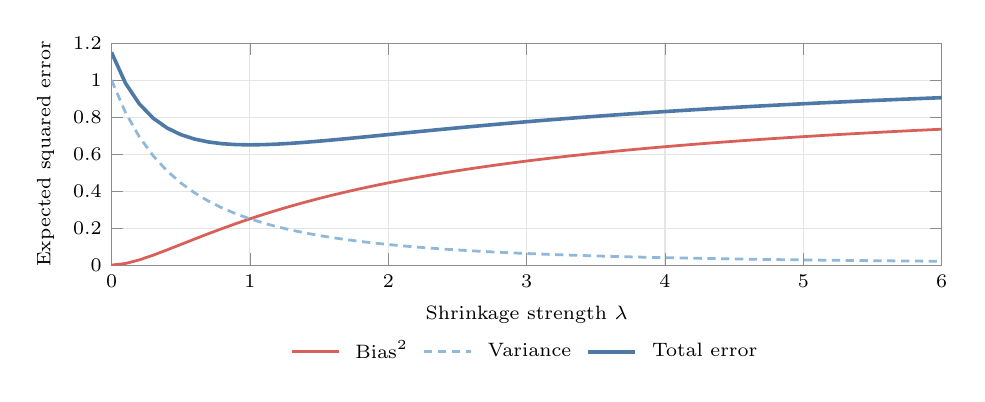
\begin{tikzpicture}
\begin{axis}[
width=\linewidth,
height=4.4cm,
font=\scriptsize,
tick label style={font=\scriptsize},
label style={font=\scriptsize},
axis line style={black!45},
tick style={black!45},
grid=major,
grid style={black!10},
xmin=0,
xmax=6,
ymin=0,
ymax=1.2,
xlabel={Shrinkage strength $\lambda$},
ylabel={Expected squared error},
scaled ticks=false,
tick label style={/pgf/number format/fixed},
clip=true,
unbounded coords=jump,
legend style={font=\scriptsize,draw=none,fill=none,at={(0.5,-0.29)},anchor=north,legend cell align=left,column sep=0.12cm,row sep=0.03cm},
legend columns=-1,
xtick={0,1,2,3,4,5,6},
ytick={0,0.2,0.4,0.6,0.8,1,1.2}
]
\addplot+[no marks,draw=redplot,line width=1pt] coordinates {(0,0) (0.1,0.00826446280992) (0.2,0.0277777777778) (0.3,0.0532544378698) (0.4,0.0816326530612) (0.5,0.111111111111) (0.6,0.140625) (0.7,0.16955017301) (0.8,0.197530864198) (0.9,0.224376731302) (1,0.25) (1.1,0.274376417234) (1.2,0.297520661157) (1.3,0.319470699433) (1.4,0.340277777778) (1.5,0.36) (1.6,0.378698224852) (1.7,0.396433470508) (1.8,0.413265306122) (1.9,0.429250891795) (2,0.444444444444) (2.1,0.45889698231) (2.2,0.47265625) (2.3,0.485766758494) (2.4,0.498269896194) (2.5,0.510204081633) (2.6,0.521604938272) (2.7,0.532505478451) (2.8,0.542936288089) (2.9,0.552925706772) (3,0.5625) (3.1,0.571683521713) (3.2,0.580498866213) (3.3,0.588967009194) (3.4,0.597107438017) (3.5,0.604938271605) (3.6,0.61247637051) (3.7,0.619737437755) (3.8,0.626736111111) (3.9,0.63348604748) (4,0.64) (4.1,0.646289888504) (4.2,0.652366863905) (4.3,0.658241367035) (4.4,0.663923182442) (4.5,0.669421487603) (4.6,0.674744897959) (4.7,0.679901508156) (4.8,0.684898929845) (4.9,0.689744326343) (5,0.694444444444) (5.1,0.699005643644) (5.2,0.703433922997) (5.3,0.70773494583) (5.4,0.7119140625) (5.5,0.715976331361) (5.6,0.719926538108) (5.7,0.723769213633) (5.8,0.727508650519) (5.9,0.731148918294) (6,0.734693877551)};
\addlegendentry{Bias$^2$}
\addplot+[no marks,draw=lightplot,line width=1pt,densely dashed] coordinates {(0,1) (0.1,0.826446280992) (0.2,0.694444444444) (0.3,0.591715976331) (0.4,0.510204081633) (0.5,0.444444444444) (0.6,0.390625) (0.7,0.346020761246) (0.8,0.308641975309) (0.9,0.277008310249) (1,0.25) (1.1,0.226757369615) (1.2,0.206611570248) (1.3,0.189035916824) (1.4,0.173611111111) (1.5,0.16) (1.6,0.147928994083) (1.7,0.137174211248) (1.8,0.127551020408) (1.9,0.118906064209) (2,0.111111111111) (2.1,0.104058272633) (2.2,0.09765625) (2.3,0.0918273645546) (2.4,0.0865051903114) (2.5,0.0816326530612) (2.6,0.0771604938272) (2.7,0.073046018992) (2.8,0.0692520775623) (2.9,0.0657462195924) (3,0.0625) (3.1,0.059488399762) (3.2,0.0566893424036) (3.3,0.0540832882639) (3.4,0.051652892562) (3.5,0.0493827160494) (3.6,0.047258979206) (3.7,0.0452693526483) (3.8,0.0434027777778) (3.9,0.0416493127863) (4,0.04) (4.1,0.0384467512495) (4.2,0.0369822485207) (4.3,0.0355998576006) (4.4,0.0342935528121) (4.5,0.0330578512397) (4.6,0.031887755102) (4.7,0.0307787011388) (4.8,0.0297265160523) (4.9,0.0287273771905) (5,0.0277777777778) (5.1,0.0268744961032) (5.2,0.0260145681582) (5.3,0.0251952632905) (5.4,0.0244140625) (5.5,0.0236686390533) (5.6,0.0229568411387) (5.7,0.0222766763199) (5.8,0.0216262975779) (5.9,0.0210039907582) (6,0.0204081632653)};
\addlegendentry{Variance}
\addplot+[no marks,draw=blueplot,line width=1.3pt] coordinates {(0,1.15) (0.1,0.984710743802) (0.2,0.872222222222) (0.3,0.794970414201) (0.4,0.741836734694) (0.5,0.705555555556) (0.6,0.68125) (0.7,0.665570934256) (0.8,0.656172839506) (0.9,0.651385041551) (1,0.65) (1.1,0.651133786848) (1.2,0.654132231405) (1.3,0.658506616257) (1.4,0.663888888889) (1.5,0.67) (1.6,0.676627218935) (1.7,0.683607681756) (1.8,0.690816326531) (1.9,0.698156956005) (2,0.705555555556) (2.1,0.712955254943) (2.2,0.7203125) (2.3,0.727594123049) (2.4,0.734775086505) (2.5,0.741836734694) (2.6,0.748765432099) (2.7,0.755551497443) (2.8,0.762188365651) (2.9,0.768671926364) (3,0.775) (3.1,0.781171921475) (3.2,0.787188208617) (3.3,0.793050297458) (3.4,0.798760330579) (3.5,0.804320987654) (3.6,0.809735349716) (3.7,0.815006790403) (3.8,0.820138888889) (3.9,0.825135360267) (4,0.83) (4.1,0.834736639754) (4.2,0.839349112426) (4.3,0.843841224635) (4.4,0.848216735254) (4.5,0.852479338843) (4.6,0.856632653061) (4.7,0.860680209295) (4.8,0.864625445898) (4.9,0.868471703533) (5,0.872222222222) (5.1,0.875880139747) (5.2,0.879448491155) (5.3,0.882930209121) (5.4,0.886328125) (5.5,0.889644970414) (5.6,0.892883379247) (5.7,0.896045889953) (5.8,0.899134948097) (5.9,0.902152909053) (6,0.905102040816)};
\addlegendentry{Total error}
\end{axis}
\end{tikzpicture}
\endgroup
